
\chapter{Números complejos}

\section{Introducción} 
Vamos a interntar resolver $x^2 + 9 = 0 \dimplies x^2 = -9 \dimplies x=\sqrt{-9}$. Siempre hemos dicho que no tiene solución. Pero yo podría escribir $(\sqrt{-9})^2 + 9 = 0$. Es decir, $\sqrt{-9}$ es solución de la ecuación. ¡Y también lo es $x_2=-\sqrt{-9}$!

La manera de trabajar con raíces negativas es sacar todos los factores hasta dejar simplemente $\sqrt{-1}$, es decir: $\sqrt{-9} = \sqrt{9}\sqrt{-1} = \pm3\sqrt{-1}$ y escribimos $\sqrt{-1} = i$. \textbf{Conclusión:} las soluciones de la ecuación son $x_1 = 3i$ y $x_2 = -3i$.

Pongamos otro ejemplo:


¿Podríamos factorizar el polinomio $P(x) = x^2-2x+2$? El \textbf{teorema fundamental del álgebra} dice que tiene 2 soluciones, pero las 2 son complejas. Vamos a verlo

Para factorizar el polinomio calculamos sus raíces resolviendo la ecuación: $P(x) = 0$

\[x^2-2x+2 = 0 \dimplies x=\frac{2\pm\sqrt{4-4·1·2}}{2} = \frac{2\pm\sqrt{-4}}{2} = \frac{2}{2} \pm \frac{2i}{2} = 1\pm i\]

Hemos obtenido 2 raíces: $α_1 = 1+i$ y $α_2 = 1-i$. ¿Cómo quedaría el polinomio factorizado? \[P(x) = x^2-2x+2 = (x-α_1)·(x-α_2) = (x-(1+i))·(x-(1-i))\]

Primera utilidad de los números complejos: resolver ecuaciones que antes eran "imposibles" y factorizar polinomios que considerábamos irreducibles.

Hay otra utilidad más: $\sqrt[6]{64}$ tiene 4 soluciones: $\sqrt[6]{64} = \{ 2,-2,1+\sqrt{3},1-\sqrt{3},-1+\sqrt{3},-1-\sqrt{3}\}$

\section{Operaciones en $ℂ$}

Un número complejo es de la forma $z=a+bi$, donde $i=\sqrt{-1}$, y llamamos $a=Re(z)$ y $b=Im(z)$. 

\paragraph{Ejemplos}
\begin{itemize}
	\item $z_1 = 3$ $\to$ $Re(z_1) = \;\;\quad\quad\;\;\;$; $Im(z_1) = \;\;\;\;\;\;\;$ \footnote{Luego, todos los números reales son complejos.}
	\item $z_2 = 2-i$ $\to$ $Re(z_2) = \;\;\quad\quad\;\;\;$; $Im(z_2) = \;\;\;\;\;\;\;$
	\item $z_3 = \sqrt{2}+6i$ $\to$ $Re(z_3) = \;\;\quad\quad\;\;\;$; $Im(z_3) = \;\;\;\;\;\;\;$
\end{itemize}

\paragraph{Representación gráfica:} como los vectores en física, sólo que aquí no hay $\vec{i}$ ni $\vec{j}$. El eje $y$ es el eje \textit{imaginario} y el eje $x$ es el eje \textit{real}.

\begin{example} Representa los números complejos $z_1 = 1-i;\;z_2 = 0;\; z_3 = 2+3i$.

\begin{figure}[hbtp]
\centering
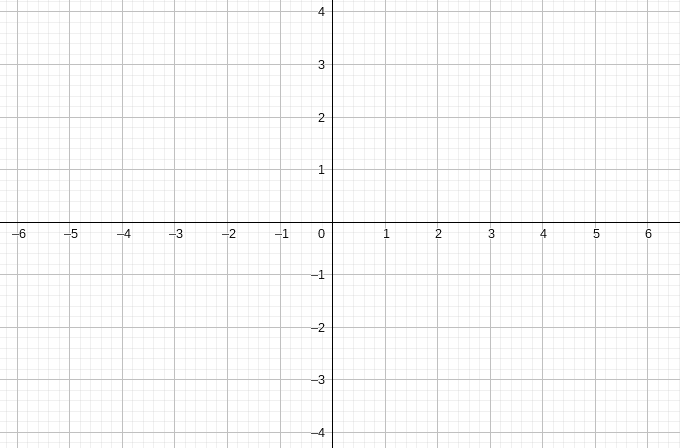
\includegraphics[scale=0.5]{../grid.png}
\end{figure}
\end{example}

\begin{defn}[Complejos\IS Conjugado] Llamamos conjugado de un número complejo $z = a+bi$ a $\bar{z} = a-bi$.

\obs Los conjugados son simétricos respecto del eje $x$.
\end{defn}

\subsection{Operaciones en forma binómica} 

\[
[(2+i)+(3-2i) - (-2i)]·[(\rfrac{1}{5}+i)] = ...
\]

\paragraph{División}

Para dividir $z_1 = a+bi$ entre $z_2 = c+di$ hacemos:

\[
\frac{z_1}{z_2} = \frac{a+bi}{c+di} = \frac{a+bi}{c+di} \frac{c-di}{c-di} = \frac{z_1}{z_2}·\frac{\bar{z_2}}{\bar{z_2}}
\]

¿Por qué se multiplica por el conjugado? En la división buscamos $z_? = x+yi$ tal que:

\[\frac{z_1}{z_2} = \frac{a+bi}{c+di} = x+yi\]

Al multiplicar arriba y abajo por el conjugado estamos quitando el número complejo del denominador. De esa manera, operando podemos obtener $x$ e $y$.


\textbf{Ejemplo: }


\paragraph{Practicar con el ejercicio 8} 

\subsubsection{Forma polar}


\begin{example}
 $z = 1-i$, dibujando el punto y sacando el ángulo que forma. 

$|z| = \sqrt{1^2+1^2} = \sqrt{2}$

$\alpha_z = \frac{-\pi}{4}$

$z = 1-i = \sqrt{2}_{\rfrac{-\pi}{4}}$

\end{example}

En la representación gráfica de números complejos, podemos utilizar otro sistema de referencia: \textit{módulo} $|z|=r$ y \textit{argumento (ángulo)} $\arg{z} = α$. 
%
Estas son las \concept[Coordenadas polares complejos]{coordenadas polares} de un número complejo y escribimos $z = r_α$


Sea $z=a+bi \in\mathbb{C}$, definimos \concept[Complejos\IS Módulo]{módulo} como $|z| = +\sqrt{a^2+b^2}$.

\obs La representación geométrica del módulo es la distancia hasta el origen de coordenadas.

Sea $z=a+bi \in\mathbb{C}$, definimos \concept[Complejos\IS Argumento]{argumento} como $\alpha = \arctg\left(\frac{Im(z)}{Re(z)}\right)$.


\textbf{Escribe en forma polar:}
\begin{itemize}
	\item $z_1 = 1+i$
	\item $z_2 = 1-i$
	\item $z_3 = 6i$
	\item $z_4 = -2-\sqrt{3}i$
\end{itemize}

\paragraph{Transformación de forma polar a binómica} Dado $z = r_α$, las coordenadas en el plano del número complejo son $(r\cos(α),r\sin(α))$, por lo que podemos escribir:

\[z = \underbrace{r_{α}}_{\text{Polar}} = \underbrace{r·(\cos(α) + i\sin(α))}_{\text{Trigonométrica}} = \underbrace{r\cos(α)}_{a}+\underbrace{r\sin(α)}_{b}i = \underbrace{a+bi}_{\text{Binómica}}\]

\paragraph{Operaciones en forma polar y trigonométrica}

Sean $z_1 = r_α$ y $z_2 = s_β$

$z_1\pm z_2$ necesitamos pasar a forma binómica/trigonométrica. ¿Para qué sirve esta forma entonces? Para multiplicar y dividir, que se hace realmente sencillo 

\hl{Corregir 8ef, 15 abc (solo polar)}. Introducir trigonométrica desde el ejercicio 15.

Operaciones en polar.

\textbf{Multiplicación:} $z_1·z_2 = (r·s)_{α+β} $

Ver \ref{trigon:multicomplejapolar} para la demostración.

\textbf{División:} $\frac{z_1}{z_2} = (\rfrac{r}{s})_{α-β} $

\textbf{Ejemplo}
\[\frac{3_{30}·5_{120}}{\sqrt{15}_{60}·1_{420}}\]


\[\frac{2_{120}·1_{240}}{\sqrt{2}_{60}·2_{30}}\]


\section{Radicación}

Sabemos que $\sqrt{16} = \pm 4$, ¿verdad? Y $\sqrt[4]{16} = \pm 2$, ¿no?

¿Nos habrán mentido desde pequeños sobre esto también? Siento decirte que sí. Vamos a verlo. 

Calcula:
\begin{itemize}
	\item $2^4 = 16$
	\item $(-2)^4 = 16$
	\item $(2i)^4 = 16·i^4 = 16$
	\item $(-2i)^4 = 16·i^4 = 16$ 
\end{itemize}

¡Cuatro raíces! De una manera general $\sqrt[n]{z}$ tiene $n$ soluciones. ¡Vamos a calcularlas! Y para esto es imprescindible la forma polar.

\begin{defn}[Radicación compleja]
$\sqrt[n]{z} = \{s_β\}$ con $s=+\sqrt[n]{|z|}$ y $β=\left\{\displaystyle\frac{\arg(z)+360k}{n}\;\;k\inℕ\right\}$
\end{defn}

\begin{example}
Calcula las 5 raíces de $z=1+i$

\textbf{Solución}
\begin{itemize}
	\item Forma polar: $z=1+i = \sqrt{2}_{45}$
	\item Las raíces serán de la forma $s_β$ con $s=\sqrt[5]{\sqrt{2}}$ y $β=\frac{45+360k}{5}$
	\begin{itemize}
		\item $k=0\to \sqrt[10]{2}_{9}$
		\item $k=1\to \sqrt[10]{2}_{81}$
		\item $k=2\to \sqrt[10]{2}_{153}$
		\item $k=3\to \sqrt[10]{2}_{225}$
		\item $k=4\to \sqrt[10]{2}_{297}$
	\end{itemize}
\end{itemize}
\end{example}


